\chapter{Research questions and Methodology}
% Methodology:
% - How do we answer RQs: simulation, controlled experiments, etc.

\section{Formalization of recurrent change detection}
Recurrent events reoccur over time with a pattern.
Pattern means the known or estimated distribution of waiting, or, inter-arrival time between successive events.
For example in the Bernoulli trials the waiting time between events has a geometric distribution.
The waiting time up to $k$-th event is a sum of $k$ independent variables.

With regard to change point detection and CD anticipation and adaptation it means that we perform an action if we expect change or CD event soon.

The main RQ is not to predict occurence, but to adapt detector or CD handling mechanism.
If sensitivity of the detector is increased than according to ARL properties, FA probability increases.
In case of model adaptation FA might
How do we adapt detector 


\section{Research questions}
% Nikolai: - Questions about ROI and PCCF
% Nikolai: - Questions about integration with detectors
% Nikolai: - Questions about impact of better detection of recurrent changes on model adaptation / adaptive learning
% Nikolai: - From the SDM, BLPA and the submitted journal paper please extract /formulate the main research questions they answer and add them here to Section 3.2

\begin{enumerate}
  \item How to formalize recurrency phenomena?
  \item How to integrate predictive confidence change function (Pccf) into change detectors?
  \begin{itemize}
    \item Post- or pre-processing settings? When and what is the safest strategy? And what are the trade offs?
    \item How to take into account uncertainty in parameters estimation (assumptions)?
  \end{itemize}
  \item What is an effect on model adaptation?
\end{enumerate}

How FA affect performance?

Change point detection in time series data and change point detection as drift detection method (DDM) as a control unit in adaptive ML system~\ref{fig:fig3_gama_survey_cd}.
Concept drifts are usually assumed to be not predictable.
We consider the case when they are predictable.
When predicting occurrence of a change point or CD event a number of assumptions is made.
Namely
\begin{itemize}
  \item The main assumption is an assumption about probability distribution of inter-arrival times between changes or CD events, and particular choice of parameters values of the distribution. 
  \item Assumptions about width of the region of interest (ROI) and its positioning relatevely to the changepoint (left, center, right).
  \item Assumption about number of events to be predicted, as with larger number the larger the uncertainty is due to mathematical properties of predictive confidence change function (Pccf).
\end{itemize}
What will happen if assumptions are wrong? And what are the benefits if correct?

Recurrency for change detection and recurrency for model adaptation.

Assumptions about statistical properties of the input signal for change detector. 

In this work we concentrate on the Change detection control unit (Figure~\ref{fig:fig3_gama_survey_cd}) which makes a decision when to retrain the model.
Implementation is done in a form of change detection algorithms.
In~\cite{XXX} we demonstrated how FA rate and detection delays can be lowered for changedetection problem if assumptions are correct.
It can be used for concept drift handling in on-line learning under certain assumptions.

\begin{itemize}

  \item Usually changes, or, concept drifts, are assumed to be not predictable. In this thesis we address to the question - can we increase change detection and prediction performance using information about temporal re-occurence patterns of changes? 

  \item How to formalize recurrency? As any sequence of events can be considered as recurrent. Answer - Assumptions about distributions of inter-arrival times.

  \item How to integrate Pccf with change detectors? What are the advantages / drawbacks of  Post- or pre-processing settings? Answer: detection delay reductions is possible only in pre-processing settings; Post-processing is more safe and only removes FAs.

  \item How to deal with uncertainty in assumptions? Answer - BLPA

  \item Assuming i) Model ii) Model with DDM iii) Model with DDM and embedded Pccf. Is it so that iii) is better than ii) and ii) is better than i) under certain assumptions (Figure~\ref{fig:research_question})? If assumptions are wrong then even ii) is not better than i)~\cite{SouzaRMB20}.

  \item What happens if Pccf predictions are not correct due to the data properties or due to the wrong assumptions/model? 

  \item How it can be used for model adaptation?

\end{itemize}

\begin{figure}[htb!]
	\centering
	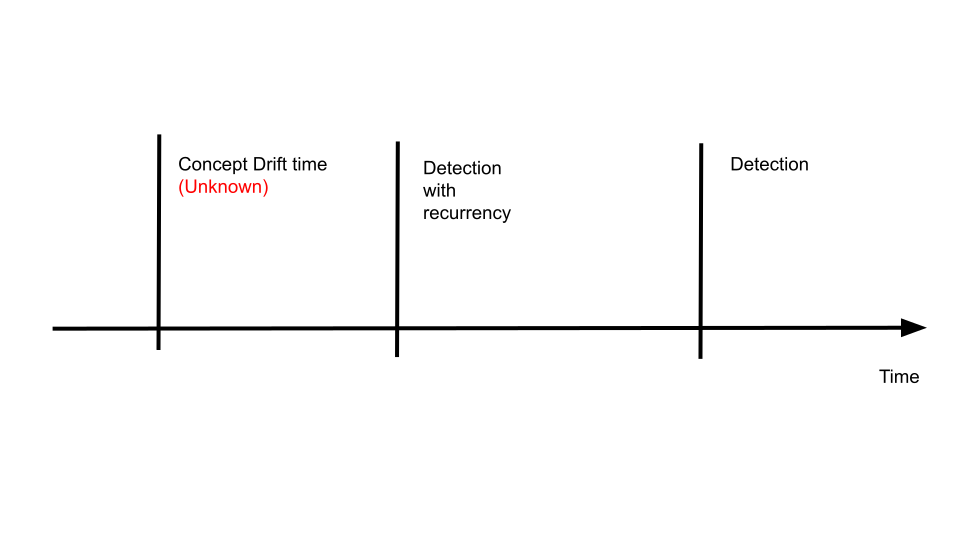
\includegraphics[width=0.9\textwidth]{images/google_slides/scheme_cd_recurrency}
  \caption{
	}\label{fig:research_question}
\end{figure}


\section{Research methodology}
%Nikolai:  Here, I think you can use a high-level umbrella or Nunamaker et al. 
%Nikolai:  See e.g. Figure 14 and brief discussion around it in my thesis at p.49  
% https://jyx.jyu.fi/bitstream/handle/123456789/13253/1/9513922715.pdf
%Nikolai:  You can adapt the figure to your needs. I.e. four ovals become:
%Nikolai:  Theory building: PCCF; (conceptualization, formalization, theorem proving
%Nikolai:  Artifact development: Recurrent change detection technique development
%Nikolai:  Experimentation with benchmark datasets: (recurrent) change detection performance; effect of (recurrent) change detection on predictive modeling
%Nikolai:  
%Nikolai:  Simulation with synthetic data: (recurrent) change detection performance
%Nikolai:  Please put as much info into Chapter 3 as you can during tomorrow. 

Figure~\ref{fig:methodology} depicts life cycle: Mathematical model; Computer simulation; Experimentation with real data sets; Field study / Deployment.
According to~\cite{nunamaker1990systems} developed system is a proof-of-concept for the research life cycle and provides an artifacts that become a subject for expanded and continuing research.
In our case Pccf construction is part of "Theory Building" and integration of Pccf with existing detectors is "Experimentation" block.
A pivotal in our work role plays computer simulations investigate detectors behavior (e.g. ARL) and effects of integration of Pccf with detectors.
Analytical - Pccf construction.
Computer simulation and experimentation - integration of Pccf with detectors.
Computer simulation is very important in this work as even, e.g. ARL estimation is quite challenging task (cite).
And often the easiest approach to answer the question , e.g. what would the expected detection delay given statistical properties of the input data, is to run a computer simulation. 

\begin{figure}[htb!]
\centering
\includestandalone[width=0.99\textwidth]{images/tikz/methodology}
  \caption{Adaptation of the diagram from~\cite{nunamaker1990systems}. Field and case studies, and deployment are parts of the future work. The first step in the }
  ~\label{fig:methodology}
\end{figure}

\begin{itemize}
  \item 1
  \item CFB in~\cite{x}
  \item Temperature signal from sensor
\end{itemize}

\section{Datasets}

In papers~\cite{MaslovSDM2016, MaslovIJCNN2017} we performed experiments experiments with artificially generated and with real datasets.

In the paper~\cite{MaslovSDM2016} we did experiments with two real datasets - with i) the boiler dataset containing sensor readings measuring recurrent refuelling behavior and ii) Internet traffic dataset\footnote{\url{https://datamarket.com/data/list/?q=internet+traffic+data+price\%3Afree}} containing aggregated internet traffic data from Internet Service Provider in the UK academic network backbone. The data series is illustrate in Figure~\ref{fig:trafficdata}.

In the paper~\cite{MaslovIJCNN2017} we used the Human activity data set~\cite{reyes2016transition} which contains sensor measurements from people performed 6 types of activities: three static postures (standing, sitting, lying) and three dynamic activities (walking, walking downstairs and walking
upstairs).

In the Journal version paper (cite) we did experiments with the time series of temperature measurements collected from the sensor installed in the home office environment.


